\documentclass[usenames,dvipsnames,notes,11pt,aspectratio=169]{beamer}
\usepackage{ifthen}
\usepackage{xcolor}
\usepackage{pgfplots}
\usepackage{amsmath}
\usepackage{centernot}
\usepackage{pifont}
\usepackage{tabularx}
\usepackage{makecell}
\usepackage{cuted}
\usepackage{booktabs}
\usepackage{array}
\usepackage{setspace}
\usepackage{CJKutf8}
\usepackage{textcomp}
\usepackage{subcaption}
\usepackage{inconsolata}
\usepackage{xspace}
\usepackage{pdfcomment}
%\newcommand{\pdfnote}[1]{\marginnote{\pdfcomment[icon=note]{#1}}}
\newcommand{\pdfnote}[1]{}

\pgfplotsset{compat=1.17}

\input ../beamer-style
\input ../std-macros
\input ../macros

\AtBeginSection[]
{
    \begin{frame}
        \frametitle{Table of Contents}
        \tableofcontents[currentsection]
    \end{frame}
}



\title[CSCI-GA.2590]{Course Overview}
\author[He He]{He He
}
\institute[NYU]{
    
\includegraphics[height=1cm]{../figures/nyu-logo}\\
}
\date{January 24, 2023}

%\includeonly{conclusion}
%\includeonlyframes{current}

\begin{document}

\begin{frame}
\titlepage
\end{frame}

\section{Logistics}

\begin{frame}
{Logistics}
            \begin{tikzpicture}
                \node[circle,draw,inner sep=0.7cm,label=below:He He (lecturer),
                    path picture={
                        \node at (path picture bounding box.center){
                            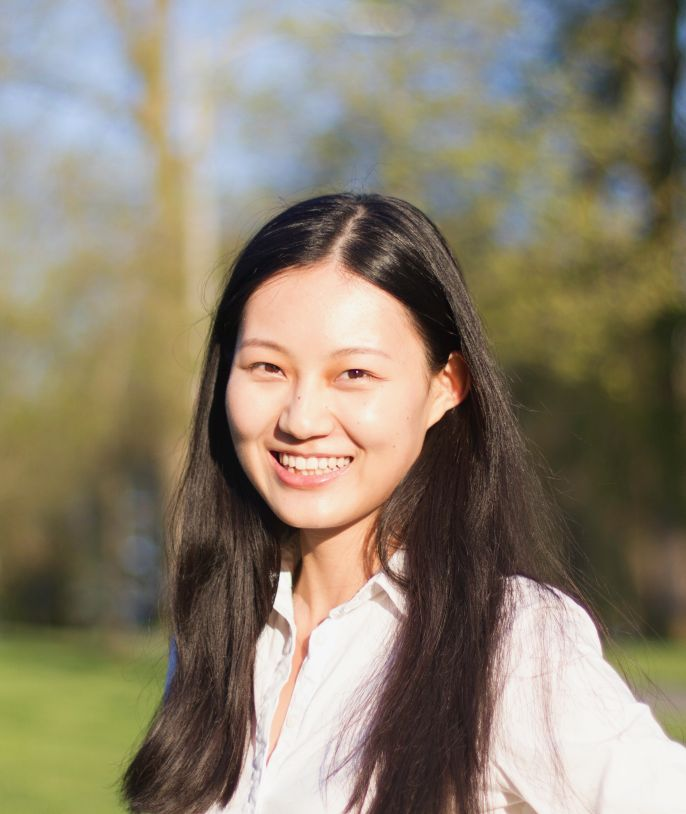
\includegraphics[width=3cm]{figures/hehe.jpg}
                        };
                    }] at(-3,0){};
                \node[circle,draw,inner sep=0.7cm,label=below:Nitish Joshi (TA),
                    path picture={
                        \node at (path picture bounding box.center){
                            
\includegraphics[width=2.5cm]{figures/nitish.jpeg}
                        };
                    }](gaomin) at (0, 0) {};
                \node[circle,draw,inner sep=0.7cm,label=below:Aditya Kashilkar (grader),
                    path picture={
                        \node at (path picture bounding box.center){
                            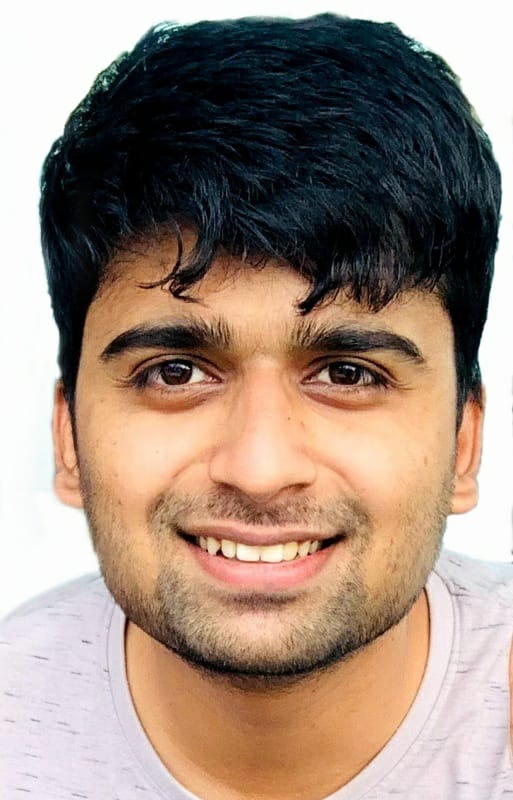
\includegraphics[width=2.5cm]{figures/aditya.jpeg}
                        };
                    }](shivesh) at (3.5, 0) {};
                \node[circle,draw,inner sep=0.7cm,label=below:Aayush Agrawal (grader),
                    path picture={
                        \node at (path picture bounding box.center){
                            
\includegraphics[width=2cm]{figures/aayush.jpg}
                        };
                    }](gauri) at (8, 0) {};
            \end{tikzpicture}
            \medskip
    \begin{itemize}
        \item Best way to communicate with us: \textbf{Campuswire} (link and code on Brightspace).
        \item Office hours will be on Zoom (details on website), or in person by appointment.
        \item Midterm will be online through Gradescope.
        \item Let us know if you have accessibility needs.
    \end{itemize}
\end{frame}

\begin{frame}
    {What this course is (not) about}
    \begin{itemize}
        \itemsep1em
        \item It's not about specific NLP applications (QA, dialogue etc.)
            \begin{itemize}
        \item Unified approaches to various NLP problems
        \item Hands-on experience in building NLP systems through assignments and the course project
            \end{itemize}

        \item It's not about fundamental machine learning
            \begin{itemize}
        \item Focus on unique challenges in language data
        \item Formalize NLP tasks as statistical learning problems
            \end{itemize}

        \item Changes from previous offerings 
            \begin{itemize}
                \item[$-$] Structured prediction (HMM, PCFG, CRF)
                \item[$+$] Large language models
            \end{itemize}
    \end{itemize}
\end{frame}

\begin{frame}
    {What we expect you to know}
    \begin{itemize}
        \itemsep1em
        \item \textbf{Linear algebra}: vector space, vector norm, dot product, gradient etc.
        \item \textbf{Probability and statistics}: conditional probability, expectation, Bayes rule etc.
        \item \textbf{Basic machine learning}: loss function, gradient descent, logistic regression etc.
        \item \textbf{Programming}: read and write Python code, use Numpy, HPC, and deep learning libraries (Pytorch, Huggingface etc.)
    \end{itemize}
\end{frame}

\begin{frame}
    {Course project}
    An important component of the course (more on this later)
    \begin{itemize}
        \itemsep1em
        \item Related to NLP (doesn't have to be in the scope of this course)
        \item New algorithms or models for existing problems
        \item Applications of NLP or ML techniques to a problem
        \item Analysis of well-known approaches that leads to new insight
        \item ML Reproducibility Challenge 2021 (\url{https://paperswithcode.com/rc2021}) 
    \end{itemize}
\end{frame}

\section{A brief history}
\begin{frame}
    {Products powered by NLP technologies}
    \begin{tikzpicture}
        \node (translation) {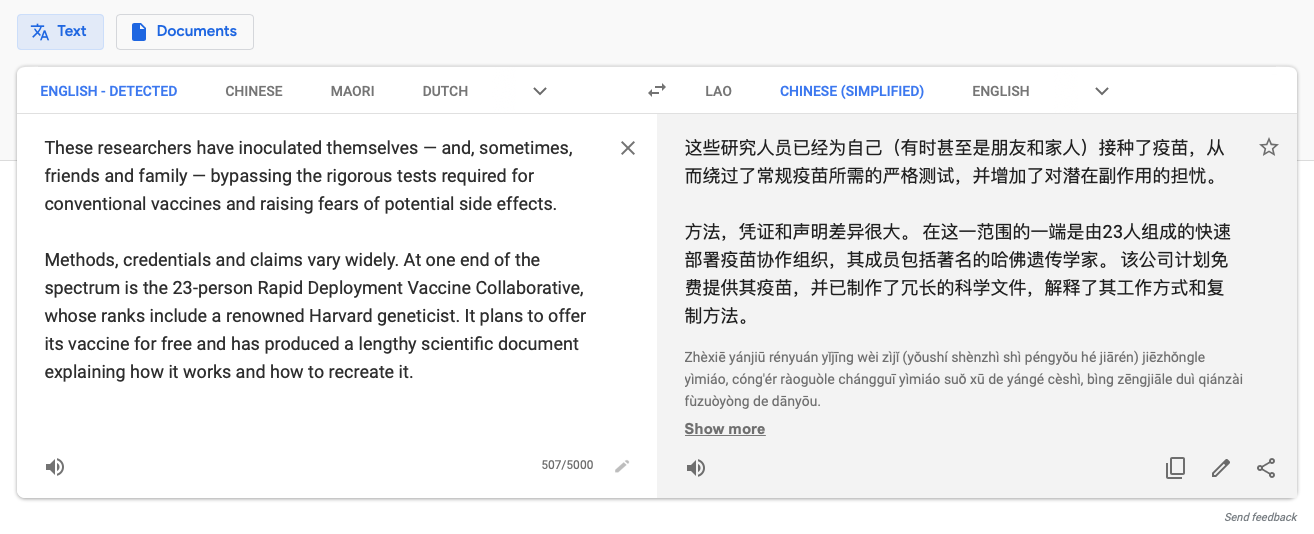
\includegraphics[width=10cm]{figures/google-translate}};
        \node (qa) [below= of translation, anchor=north east, yshift=3em]{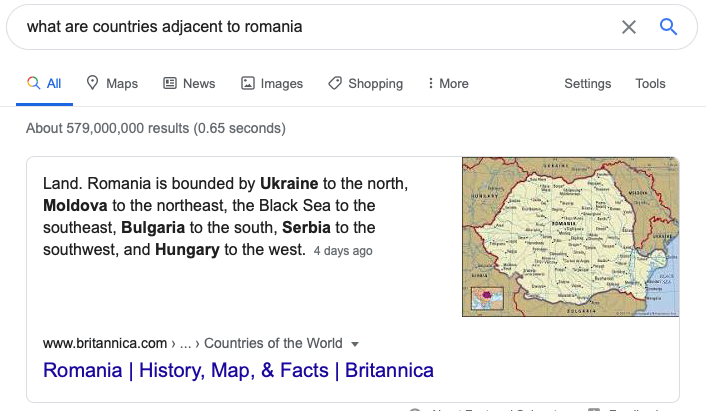
\includegraphics[width=5cm]{figures/search-qa}};
        \node [right= of qa]{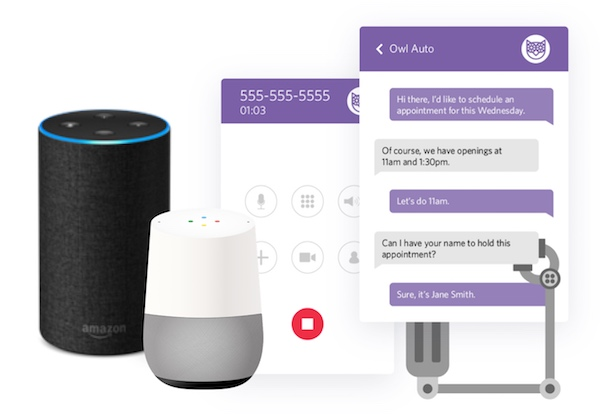
\includegraphics[width=5cm]{figures/alexa}};
    \end{tikzpicture}
\end{frame}

\begin{frame}
    {A single natural language interface for everything}
    \begin{figure}
        
\includegraphics[width=10cm]{figures/chatgpt-1}
    \end{figure}
\end{frame}

\begin{frame}
    {A single natural language interface for everything}
    \begin{figure}
        
\includegraphics[width=10cm]{figures/chatgpt-2}
    \end{figure}
\end{frame}

\begin{frame}
    {Language is at the core of AI: the imitation game}
    \begin{figure}
        \begin{subfigure}[b]{0.4\textwidth}
        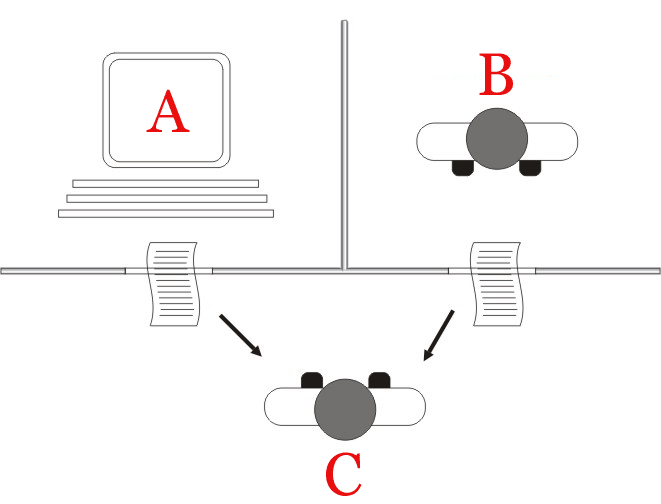
\includegraphics[height=3cm]{figures/turing-test}
        \end{subfigure}\hfill
        \begin{subfigure}[b]{0.4\textwidth}
        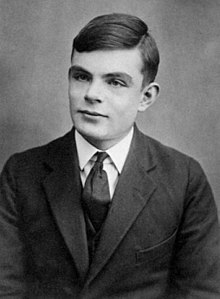
\includegraphics[height=4cm]{figures/turing}
        \end{subfigure}
    \end{figure}
    \pdfnote{The interrogator chats with two agents and must tell which is human vs AI.}

    \nl{I believe that in about \blue{fifty years'} time it will be possible to programme computers, with a \blue{storage capacity of about $10^9$}, to make them play the imitation game so well that an average interrogator will not have more than 70 percent chance of making the right identification after five minutes of questioning.} Turing (1950)
    %I believe that at the end of the century the use of words and general educated opinion will have altered so much that one will be able to speak of machines thinking without expecting to be contradicted.'' 

    \pause\medskip
    \think{Is humanlikeness the ultimate goal?}
    \pdfnote{You can have a not so smart AI which an fake humanlikeness, or a superhuman AI that can be detected by the interrogator.}
\end{frame}

\begin{frame}
    {ELIZA}
    \begin{itemize}
        \item Built by Joseph Weizenbaum at MIT in 1964 to demonstrate the \emph{superficiality} of human-machine communication.
        \item Surprisinly, people were convinced that ELIZA had human intelligence.
    \end{itemize}
    \bigskip
    \centering
    \begin{table}
        \begin{tabular}{ll}
            Human: & Well, my boyfriend made me come here.\\
    ELIZA: & Your boyfriend made you come here?\\
    Human: & He says I'm depressed much of the time.\\
    ELIZA: & I am sorry to hear you are depressed.\\
    Human: & It's true. I'm unhappy.\\
    ELIZA: & Do you think coming here will help you not to be unhappy?
        \end{tabular}
    \end{table}
\end{frame}

\begin{frame}
    {Early rule-based systems: the Georgetown-IBM experiment}
    \begin{itemize}
        \item The Russian-English machine translation program:\\
            \begin{center}
            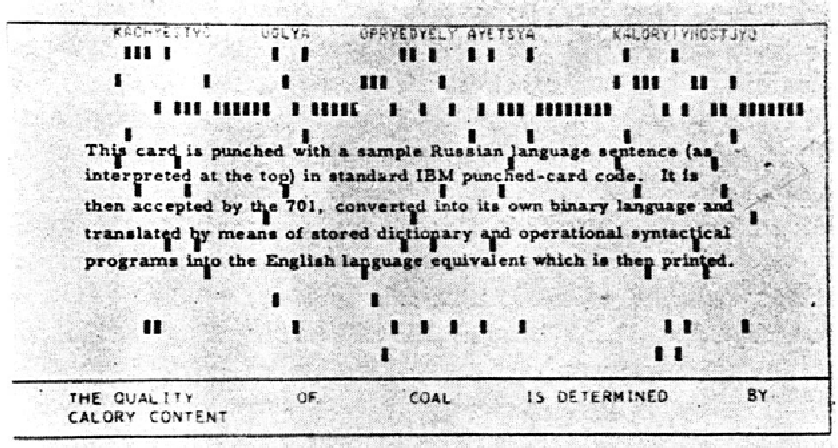
\includegraphics[height=3cm]{figures/ibm-experiment}
            \end{center}
        \item A vocabulary of \blue{250 words}
        \item Using \blue{6 grammar rules}, \eg\\
            \texttt{
                If first code is 110, is third code associated with preceding complete word equal to 21? If so, reverse order of appearance of words in output (i.e., word carrying 21 should follow that carrying 110)---otherwise, retain order.}
    \end{itemize}
\end{frame}

\begin{frame}
    {Approaching AI as a whole: SHRDLU}
    \begin{columns}
        \begin{column}{0.6\textwidth}
    \begin{itemize}
        \item Built by Terry Winograd at MIT in 1968.
        \item A person instructs the computer to build structures in a blocks world.
        \item \blue{Require many capabilities}: grounding, coreference resolution, question answering, semantic parsing etc. 
    \end{itemize}
        \end{column}
        \begin{column}{0.4\textwidth}
    \begin{center}
    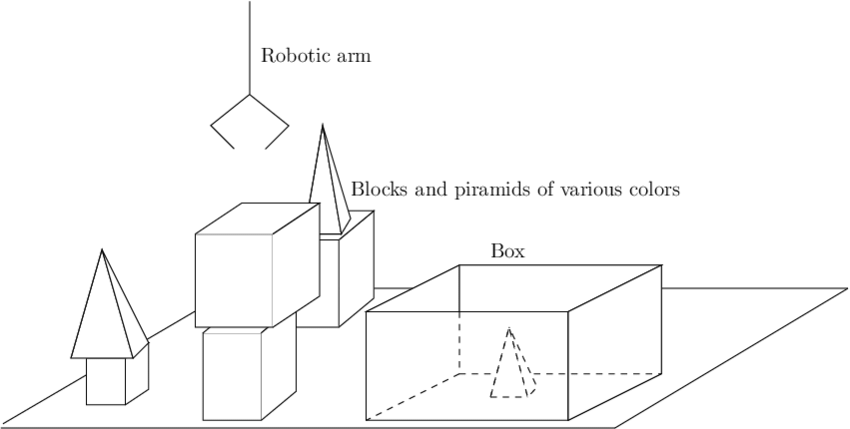
\includegraphics[height=3cm]{figures/shrdlu}
    \end{center}
        \end{column}
    \end{columns}
    \begin{table}
        \begin{tabular}{lp{12cm}}
            Person:& Pick up a big red block.\\
            Computer:& OK.\\
            Person:& Grasp the pyramid.\\
            Computer:& I don't understand which pyramid you mean.\\
            Person:& (changing their mind) Find a block which is taller than the one you are holding and put it into the box.\\
            Computer:& By "it", i assume you mean the block which is taller than the one i am holding.
    \end{tabular}
    \end{table}
\end{frame}

\begin{frame}
    {Limitations of early systems}
    \begin{itemize}
        \itemsep1em
        \item Optimism in the 50's and 60's: working on tasks that are too complex at that time\\[1ex]
            \nl{Within the very near future---much less than twenty-five years---we shall have the technical capability of substituting machines for any and all human functions in organizations.}
        \item Disappointing results due to
            \begin{itemize}
                \item \textbf{Limited computation}: hardware has limited speed and memory 
                \item \textbf{Combinatorial explosion}: algorithms are intractable in realistic settings
                \item \textbf{Underestimated complexity}: ambiguity, commonsense knowledge etc.
            \end{itemize}
    \end{itemize}
\end{frame}

\begin{frame}
    {The rise of statistical learning in the 80's}
    \begin{itemize}
        \itemsep1em
        \item Notable progress in MT from IBM (neglected knowlege of linguistics).
        \item HMMs widely used for speech recognition.\\
            \nl{Every time I fire a linguist, the performance of the speech recognizer goes up.}---Frederick Jelinek.
        \item The paradigm shift: \blue{expert knowledge + rules $\rightarrow$ data + features}
        \item Statistical learning is the main driving force of NLP today.
    \end{itemize}
\end{frame}

\begin{frame}
    {The deep learning tsunami}
    \begin{itemize}
        \itemsep1em
        \item Before deep learning (around 2015), NLP is mostly about structured prediction and feature engineering.
        \item Neural networks can automatically learn good features/representations for a task 
        \item The paradigm shift: \blue{features $\rightarrow$ network architectures + embeddings}
        \item Almost all NLP models are neural networks nowadays.
    \end{itemize}
\end{frame}

\begin{frame}
    {Models and data keep getting larger}
    \begin{itemize}
        \itemsep1em
        \item Since around 2018, Transformer-based pretrained models have become the standard. 
        \item Pre-training on large data provides useful representations for many downstream tasks.
        \item The paradigm shift: \blue{architecture design $\rightarrow$ transfer learning (fine-tuning)}
        \item More recently, a single natural language interface for all tasks (\eg ChatGPT by OpenAI).
        \item The paradigm shift: \blue{transfer learning $\rightarrow$ instructing / prompting}
    \end{itemize}
\end{frame}

\section{Challenges in NLP}

\begin{frame}
    {Why is language hard?}
    \pause
    \begin{itemize}
        \item \textbf{Discrete}
            \begin{itemize}
                \itemsep1em
                \item How to define metrics?
                    \\\medskip
                    \begin{tabular}{lcl}
                        I work \blue{at} NYU. & vs & I work \blue{for} NYU. \\
                        This is good. & vs & This is \blue{actually} good.
                    \end{tabular}
                \item How to define transformations?\\
                    \medskip
                    \begin{tabular}{p{7cm}cp{5cm}}
                    The food is okay. & $\rightarrow$ & The food is awesome! \\
                    They made a brief return to Cambridge to drop the book. & $\rightarrow$& They returned.
                    \end{tabular}
                \item In general, hard to represent text as mathematical objects.
            \end{itemize}
    \end{itemize}
    \begin{table}
    \end{table}
\end{frame}

\begin{frame}
    {Why is language hard?}
    \begin{itemize}
        \item \textbf{Compositional}
            \begin{itemize}
                \item The whole is built from parts (chars, words, sentences, paragraphs, documents...)
                \item How to generalize when we don't see all possible combinations?\\
                \item An example from \mycite{Lake et al., 2018}\\
                Vocabulary:\\
                    \begin{itemize}
                    \item[]\{jump, walk, turn, once, twice, left, right, before, after, and\}
                    \end{itemize}
                Sentences: \\
                    \begin{itemize}
                       \item[]jump \\
                       \item[]jump left\\
                       \item[]jump left and walk right \\
                       \item[]jump left after walk right once before turn left twice\\
                       \item[]...
                    \end{itemize}
            \end{itemize}
    \end{itemize}
\end{frame}

\begin{frame}
    {Why is language hard?}
    \begin{itemize}
        \item \textbf{Sparse} 
            \begin{itemize}
                \item How to handle the long tail?
                \item Zipf's law: $\text{word frequency} \propto \frac{1}{\text{rank}}$
                    \begin{figure}
                        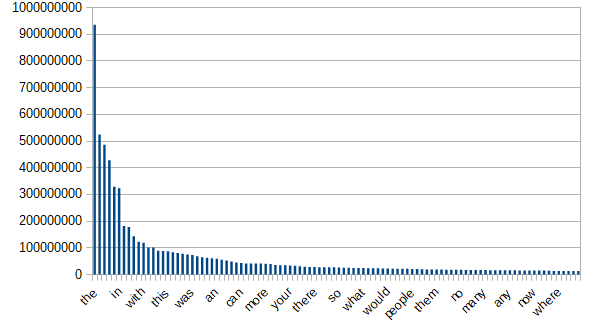
\includegraphics[height=3cm]{figures/zipf}
                    \end{figure}
                \item Many linguistic phenomena follow Zipf's law\\
                    BoA's financial assistant Erica:\\
                    \textit{The bank ``learned [that] there are over 2,000 different ways to ask us to move money.''}\footnote[frame]{
                        \url{https://www.aiqudo.com/2019/06/28/voice-success-story-erica-bank-america/}
                    }
            \end{itemize}
    \end{itemize}
\end{frame}

\begin{frame}
    {Why is language hard?}
    \begin{itemize}
        \item \textbf{Ambiguous} 
            \begin{itemize}
                \item How to interpret meaning in context?
                \medskip
                \begin{itemize}
                    \itemsep2em
                    \item[] Bass: fish? guitar? frequency? (word sense disambiguiation)
                    \item[] I shot an elephant in my pajamas: who is in the pajamas? (PP attachment)
                    \item[] The spirit is willing but the flesh is weak.\\
                        $\rightarrow$ 
                        The vodka is strong but the meat is rotten.
                \end{itemize}
            \end{itemize}
    \end{itemize}
\end{frame}


\end{document}
